\documentclass[10pt,twocolumn,letterpaper]{article}

\usepackage{3dv}
\usepackage{times}
\usepackage{epsfig}
\usepackage{graphicx}
\usepackage{amsmath}
\usepackage{amssymb}

% Include other packages here, before hyperref.

% If you comment hyperref and then uncomment it, you should delete
% egpaper.aux before re-running latex.  (Or just hit 'q' on the first latex
% run, let it finish, and you should be clear).
\usepackage[pagebackref=true,breaklinks=true,letterpaper=true,colorlinks,bookmarks=false]{hyperref}


%\threedvfinalcopy % *** Uncomment this line for the final submission

\def\threedvPaperID{****} % *** Enter the 3DV Paper ID here
\def\httilde{\mbox{\tt\raisebox{-.5ex}{\symbol{126}}}}

% Pages are numbered in submission mode, and unnumbered in camera-ready
\ifthreedvfinal\pagestyle{empty}\fi
\begin{document}

%-------------------------------------------------------------------------
%%%%%%%%% TITLE
\title{Plant Leaf Meshes from RGB-D Sensors}

\author{ 
Daniel Morris \and Saif Imran \and Vincent Zickefoose \and Jin Chen \and David Kramer\\
%Need to fix the following:
Department of Electrical and Computer Engineering\\
Department of Energy Plant Research Laboratory\\
Michigan State University, East Lansing, MI 48824, USA
}

\maketitle

%-------------------------------------------------------------------------
\begin{abstract}

\end{abstract}
%-------------------------------------------------------------------------

\section{Introduction}
\label{sec:intro}

Introduction here including application description


\section{Related Work}
\label{sec:related}




\section{Data Modeling}
\label{sec:data}

\begin{figure}
\begin{center}
%\fbox{\rule{0pt}{5in} \rule{0.9\linewidth}{0pt}}
   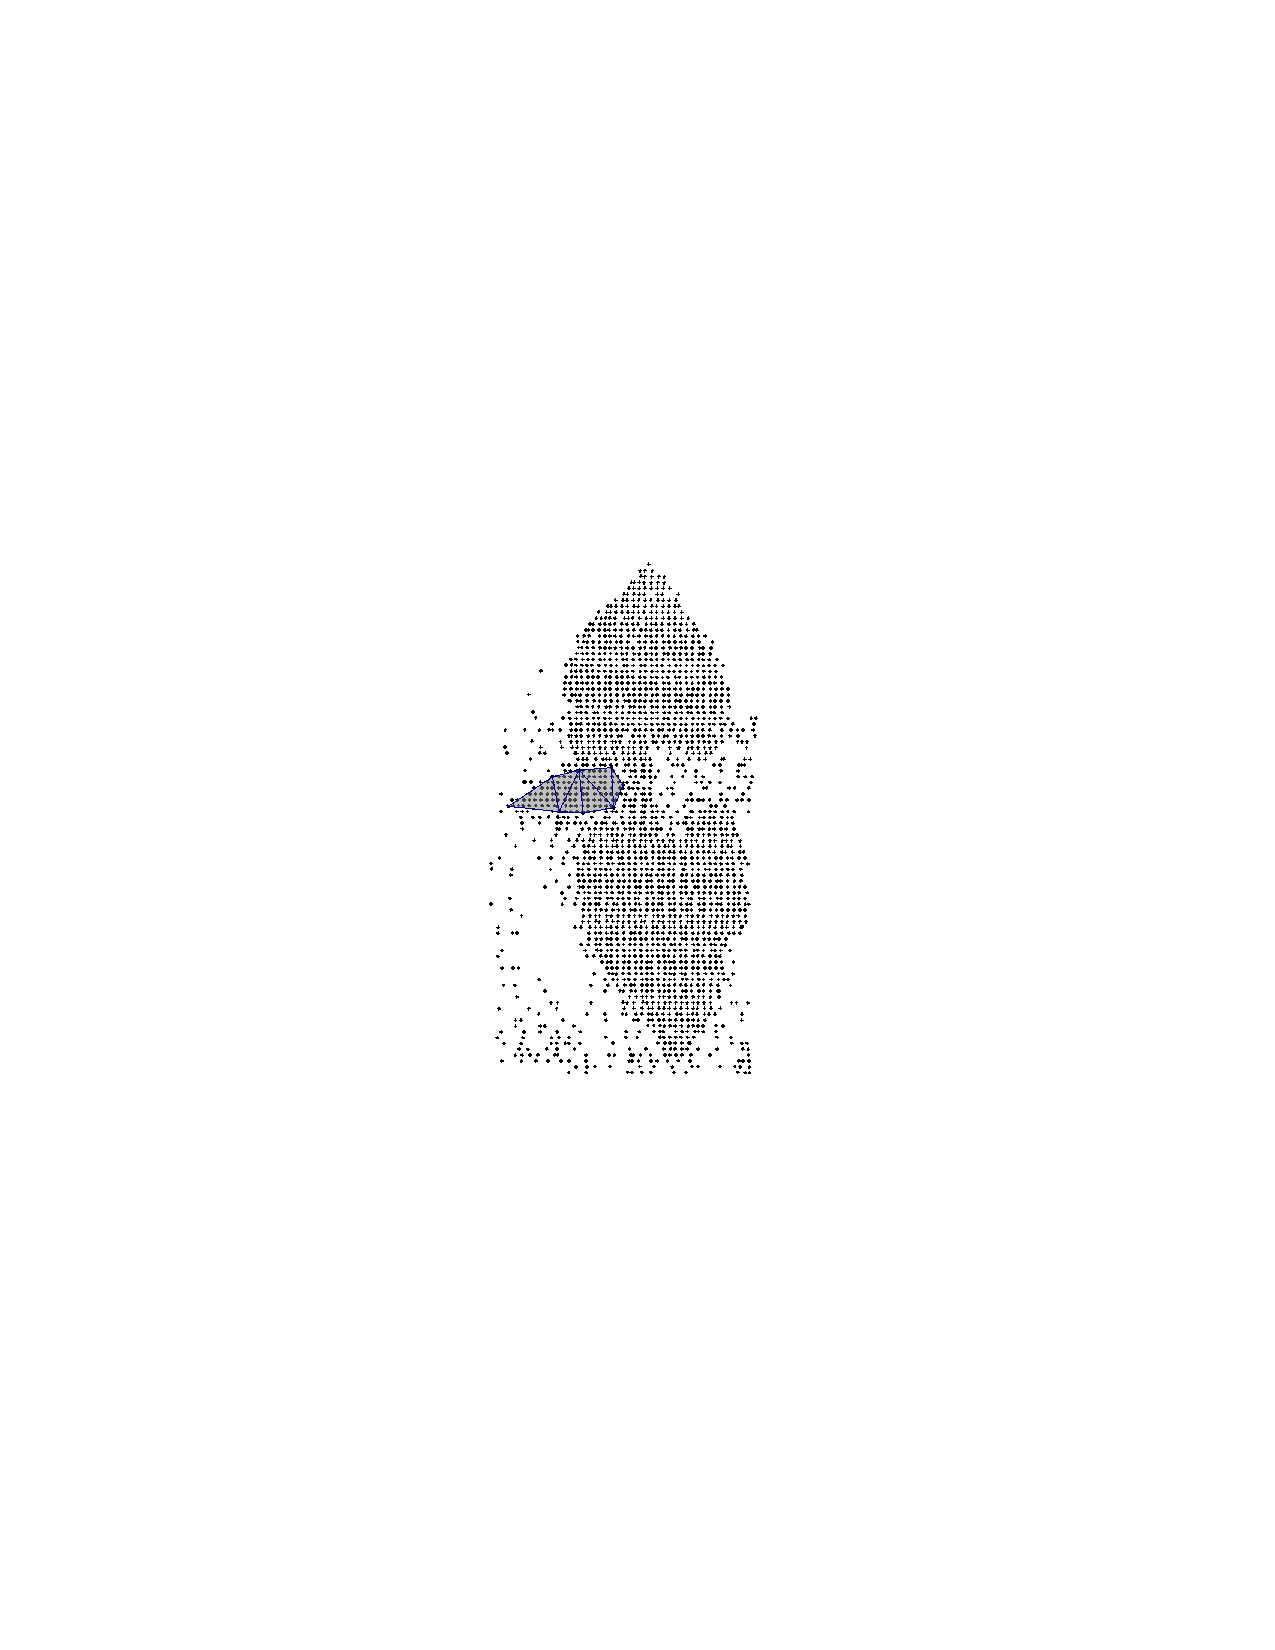
\includegraphics[trim=200 250 200 270,clip,width=0.9\linewidth]{Figures/sampleLeaf}
\end{center}
   \caption{Example caption of a leaf image with $3$D projected points.}
\label{fig:long}
\label{fig:onecol}
\end{figure}

An example citation~\cite{Zhang2000}.


\section{Mesh Formulation}
\label{sec:mesh}




\section{Results}
\label{sec:results}




\section{Conclusion}
\label{sec:conclusion}




%-------------------------------------------------------------------------

{\small
\bibliographystyle{ieee}
\bibliography{sense3d}
}
%-------------------------------------------------------------------------

\end{document}
